\begin{figure}
  \centering
  \begin{subfigure}[b]{\linewidth}
    \centering
    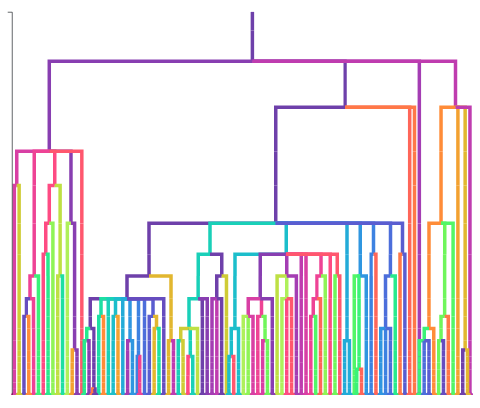
\includegraphics[width=\textwidth, height=0.16\textheight]{img/plain_resolution_3}
    \caption{33\% resolution}
    \label{fig:perfect-tree-phylometrics-sensitivity-analysis:epoch0}
  \end{subfigure}
  \begin{subfigure}[b]{\linewidth}
    \centering
    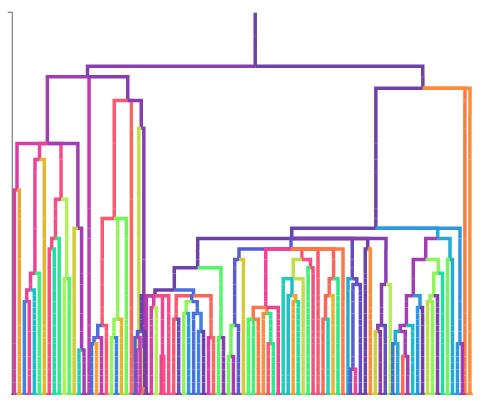
\includegraphics[width=\textwidth, height=0.16\textheight]{img/plain_resolution_10}
    \caption{10\% resolution}
    \label{fig:perfect-tree-phylometrics-sensitivity-analysis:epoch2}
  \end{subfigure}
  \begin{subfigure}[b]{\linewidth}
    \centering
    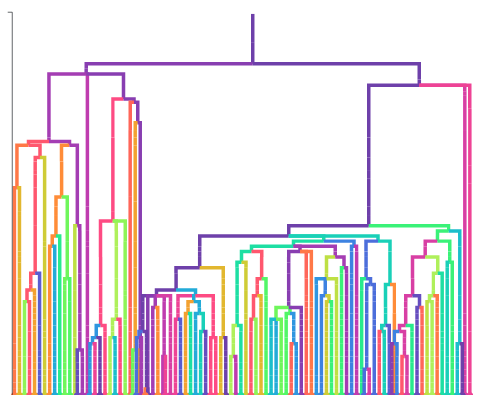
\includegraphics[width=\textwidth, height=0.16\textheight]{img/plain_resolution_30}
    \caption{3\% resolution}
    \label{fig:perfect-tree-phylometrics-sensitivity-analysis:exponential}
  \end{subfigure}
  \begin{subfigure}[b]{\linewidth}
    \centering
    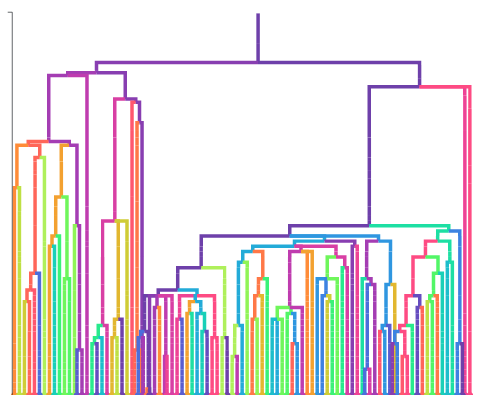
\includegraphics[width=\textwidth, height=0.16\textheight]{img/plain_resolution_100}
    \caption{1\% resolution}
    \label{fig:perfect-tree-phylometrics-sensitivity-analysis:exponential}
  \end{subfigure}
  \begin{subfigure}[b]{\linewidth}
    \centering
    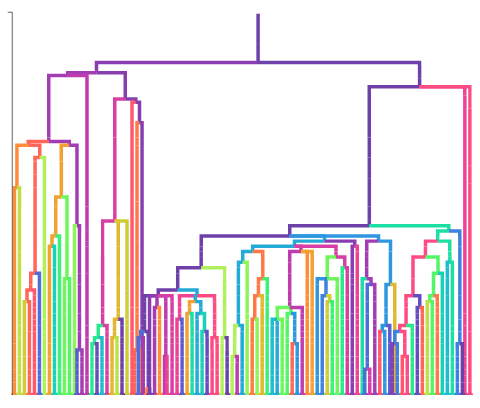
\includegraphics[width=\textwidth, height=0.16\textheight]{img/reference}
    \caption{reference tree}
    \label{fig:perfect-tree-phylometrics-sensitivity-analysis:exponential}
  \end{subfigure}
  \caption{TODO}
  \label{fig:perfect-tree-phylometrics-sensitivity-analysis}
\end{figure}
